%\section{The Unlearn--Retain Tension}
\section{Motivation}
\label{sec:motivation} 
Current concept unlearning methods are designed to suppress a concept token (e.g., ``\texttt{horse}'') 
% \varun{you used \texttt{horse} earlier; be consistent?} 
so as to remove the corresponding visual concept without substantially affecting other concepts. This design implicitly assumes that visual concepts are represented as localized, token-aligned features in the model's joint text--image space.
In this section, we present empirical evidence that this assumption fails: 
in practice, unlearning a target concept produces 
% \emph{collateral damage} to semantically neighboring concepts 
\emph{collateral damage} to the concepts with which it is entangled. 
% \footnote{We define semantic neighborhood formally in \cref{subsec:definitions} as the set of concepts whose activation regions in the model's cross-attention space lie within distance $\delta$ of the target's. In this section, ``neighbors'' refers operationally to fine-grained subtypes and near-synonyms (e.g., \texttt{donkey}, \texttt{pony} for \texttt{horse}).}
\footnote{We define entanglement formally in \cref{subsec:definitions} based on activation regions in the model's cross-attention space.}
%, and the severity of that damage is coupled to the robustness \footnote{Throughout this section, ``robustness'' refers informally to how reliably the target concept is suppressed across diverse prompts, including indirect ones that do not mention the concept word. We make this precise as $\varepsilon$-robust unlearning in \cref{def:robust}.} of the erasure. 
The severity of this damage is coupled to both the strength of the erasure applied to the target concept and the extent of its entanglement with other concepts.
This coupling is the phenomenon our theoretical framework analyzes in~\cref{sec:tradeoff}.

% diffusion models exhibit strong \emph{concept entanglement}, where semantically related concepts share overlapping representational structure. 
% This entanglement produces two observable consequences---concept leakage and collateral forgetting---that we argue are not independent failure modes but rather \emph{dual manifestations of the same underlying phenomenon}: shared representational structure across correlated concepts.

% Two observations drive this framing. First, diffusion models condition on prompt embeddings produced by text encoders that exhibit bag-of-words behavior~\citep{yuksekgonul2022and}: prompts that omit a concept token (\emph{horse}) but retain its typical context (\emph{jockey}, \emph{saddle}, \emph{racetrack}) can still induce activations associated with that concept. \varun{thus?} The visual concept is distributed across ``correlated'' context tokens, not isolated in a single word. \varun{examples? point to fig?}
%Second, semantically neighboring concepts share much of this context (\emph{``a horse in a field''}, \emph{``a donkey in a field''}), causing their activation regions to overlap \varun{so what?}. Together these observations imply that any intervention modifying the activation region of one concept will propagate to its neighbors.

The training mechanisms of text-to-image diffusion models make entanglement inevitable.
First, diffusion models condition on prompt embeddings produced by text encoders that often exhibit bag-of-words behavior~\citep{yuksekgonul2022and}. As a result, prompts that omit a concept token (e.g., \texttt{horse}) but retain its characteristic context (e.g., \texttt{jockey}, \texttt{saddle}, \texttt{racetrack})
% \varun{again, use texttt?}
can still induce activations associated with that concept (see~\cref{fig:bow_context_span}). This implies that the visual concept is not localized in a single token, but is instead distributed across multiple correlated context tokens. Second, semantically related concepts share much of this contextual structure (e.g., \emph{a horse in a field''} vs.\ \emph{a donkey in a field''}), which leads to overlapping activation regions in the model’s internal representation space.

\Cref{fig:concept_leakage} illustrates an example of the trade-off due to this entanglement. It shows two unlearning methods using \texttt{horse} as the erasure target.
% \ali{the figure does not seem to match the description here anymore?}.
Method that perform localized erasure (ESD~\cite{gandikota2023erasing}) successfully suppress generation when the target token is named, but regenerate the concept through indirect prompts that name only context words, which we call \emph{concept leakage}. 
Methods that erase more aggressively (STEREO~\cite{srivatsan2025stereo}) suppress this leakage but produce visibly degraded outputs for some semantically similar concepts, such as \texttt{donkey} and \texttt{zebra}, that are entangled with the target concept (see~\cref{tab:kappa}). We call this effect \emph{collateral damage}. 

Together, these observations imply that modifying the activation region of a target concept necessarily affects other concepts that rely on the same shared representation. In other words, interventions intended to suppress a concept will propagate to concepts with which is it entangled, giving rise to both concept leakage and collateral damage. 
%\varun{i would comment the rest of this text} In~\cref{sec:tradeoff} we formalize this constraint as a provable lower bound on the trade-off between erasure effectiveness and utility preservation. And in~\cref{sec:experiment}, we validate the trade-off quantitatively across seven unlearning methods.

\begin{comment}
    \subsection{Why Concepts Are Entangled: Distributed Representations in Diffusion Models}
\label{subsec:bow}

The roots of concept entanglement lie in how diffusion models process text. These models condition image generation on embeddings produced by pretrained text encoders (e.g., CLIP~\citep{radford2021learning}), which have been shown to exhibit \emph{bag-of-words} behavior: prompt embeddings are often well-approximated by aggregations over individual token embeddings, with limited sensitivity to word order and relational bindings~\citep{yuksekgonul2022and}.
Following this observation, we view the prompt embedding $f_\psi(p)$ as being influenced not only by the token naming a concept, but also by the surrounding context tokens that frequently co-occur with it.
% Under such a representation, if the text encoder behaves approximately as
% \begin{equation}
%     f_\psi(p) \;\approx\; \sum_{t \in p} \boldsymbol{\Phi}(t),
% \end{equation}
% where $\mathrm{Tok}(p)$ denotes the tokens in prompt $p$ \varun{where is $\mathrm{Tok}(p)$ used? should it be $t \in Tok(p)$?}, and $\boldsymbol{\Phi}(t)$ is the embedding of token $t$ \varun{why a different embedding function and not $f_\psi$?},
% then the embedding of a concept is not determined by a single token but by the \emph{constellation of co-occurring tokens} in its typical prompt context \varun{what does constellation mean in this context? also, is the equation above from yuksekgonul's paper? if so -- state it! if not, provide more justification for why it is a sum?}. 
For example, prompts involving the concept \texttt{horse} often contain context words such as \emph{rider}, \emph{saddle}, \emph{barn}, or \emph{galloping}. As a result, the model can associate the visual concept with a broader textual context rather than with a single lexical item alone.
% Training captions in large-scale text-to-image datasets reinforce this: captions containing the concept \texttt{horse} frequently include tokens such as \emph{rider}, \emph{saddle}, \emph{cowboy}, and \emph{stable} \varun{so what?}. 
For simplicity, let $t_c$ denote the token %\varun{what if horse is split into 2 tokens? state that you're making a simplifying assumption that the concept corresponds to a single token} 
corresponding to concept $c$, 
and let $S_c$ denote a set of context tokens that frequently co-occur with $t_c$ in prompts. 
Then prompts that omit $t_c$ but retain enough of $S_c$ can still produce text embeddings similar to those of prompts that explicitly contain $t_c$. At a high level, this suggests that
\begin{equation}
\label{eq:bow_approx}
\mathbb{E}[\mathbf{e}_p \mid t_c \in p]
\;\approx\;
\mathbb{E}[\mathbf{e}_p \mid S_c \subseteq p].
\end{equation}
where $\mathbf{e}_p = f_\psi(p)$ denotes the prompt embedding.

% \ali{is $\mathbf{e}_p$ same as $e_p$ in the definitions. make sure notations is consistent.}
\varun{i don't understand the equation above? it is saying that in expectation, the embeddings are the same? but maybe the RHS needs to be more specific to say that $t_c \notin p$? otherwise it is not communicating the point you want to make}

\ali{i think it might be better to use an equation that implies the image generation on the prompts from $S_c$ is almost the same. claiming that prompt embeddings are the same is not what we directly evaluate? maybe something like this:
\[
\mathbb{E}_{p \sim \mathcal{P}(t_c)} \left[\, 
\Pr_{x \sim p_\theta(\cdot \mid p)}\big[O_X(x, c) = 1\big] 
\,\right]
\;\approx\;
\mathbb{E}_{p \sim \mathcal{P}(S_c \setminus t_c)} \left[\, 
\Pr_{x \sim p_\theta(\cdot \mid p)}\big[O_X(x, c) = 1\big] 
\,\right]
\]
}

This means that the representation of concept $c$ is distributed across correlated context tokens, not isolated in a single word. 
The same logic also explains why neighboring concepts can overlap. For instance, prompts such as a horse in a field,'' a deer in a field,'' and ``a zebra in a field'' share a common contextual scaffold while differing in only one concept token.
% Crucially, neighboring concepts (e.g., \texttt{deer}, \texttt{zebra}) share many of the same contextual tokens (e.g., \emph{field}, \emph{galloping}, \emph{animal}), causing their activation regions in the model's internal representation space to overlap. 
% \varun{this is not coming across from the theory or the equations above! you may want to show that there are many prompts of a "fixed" structure where only one token varies. for example: in the farm, there is a "cow/horse/dog" etc -- and this can motivate what neighboring concepts are.} 
Because these prompts induce similar text-conditioned activations, the corresponding concepts can have overlapping regions in the model's internal representation space.
This overlap creates the fundamental tension we study: suppressing one concept by modifying the shared region can also disturb neighboring concepts that rely on the same contextual structure.%any intervention that modifies the shared representational region to suppress one concept risks disrupting its neighbors. \varun{equation 3 and 2 do not show that, so this last statement is not motivated thus far!}

\end{comment}

%\paragraph{Two Sides of the Same Coin}
% We now demonstrate that concept entanglement produces two empirically observable effects that constrain every unlearning method. These effects are not independent failure modes to be addressed separately; they are coupled consequences of representational overlap. 

%\ali{I think the section starts very abruptly with Figure 2 illustrates "the consequence" of "this" structure. what consequence? what structure? the section should be kind of self-contained. So I think either remove the hearder and merge with the previous text or add a couple of sentences at the begenning. }

%\Cref{fig:concept_leakage} illustrates the consequence of this structure using \texttt{horse} as the erasure target across two unlearning methods.
% \ali{the figure does not seem to match the description here anymore?}.
%Method that perform localized erasure (ESD~\cite{gandikota2023erasing}) successfully suppress generation when the target token is named, but regenerate the concept through indirect prompts that name only context words, which we call \emph{concept leakage}. 
%Methods that erase more aggressively (STEREO~\cite{srivatsan2025stereo}) suppress this leakage but produce visibly degraded outputs for semantically neighboring concepts such as \texttt{donkey} and \texttt{zebra} after erasing \texttt{horse}, which we consider \emph{collateral damage to neighbors}. 
% No method in our study simultaneously avoids both failures.

% \paragraph{Effect 1: Concept leakage through correlated prompts.}
% After applying each unlearning method to erase \texttt{horse}, we test whether the concept can be regenerated using prompts that omit the target token but include semantically related context. Example prompts include \emph{``Image of the animal a jockey rides at the racetrack''} and \emph{``A royal procession with decorated ceremonial mounts.''}

% As shown in Figure~\ref{fig:concept_leakage}, methods that perform lightweight or localized erasure (ESD, SAeUron) successfully suppress the concept when the token \texttt{horse} appears in the prompt, but still regenerate it for a substantial fraction of contextual prompts that omit the target token.
% \yian{Concretely, over (N) indirect prompts, ESD regenerates horse-like images in () cases, and SAeUron does so in () cases.}
% \varun{more precise? how many tries, how many successes etc.?}. 
% This is a direct consequence of Eq.~\eqref{eq:bow_approx}: the model's representation of \texttt{horse} extends beyond the token itself into a broader region of activation space populated by co-occurring tokens. Unlearning the token's direct contribution leaves this broader region largely intact.

% \paragraph{Effect 2: Collateral forgetting of neighboring concepts.}
% Methods that achieve more aggressive erasure---particularly STEREO, which uses a form of adversarial training to suppress the concept across a wide region of embedding space---substantially reduce concept leakage. However, this robustness comes at a cost. After erasing \texttt{horse} with STEREO, we observe significant degradation in the model's ability to generate semantically neighboring concepts. Prompts such as \emph{``a deer standing in a forest''} and \emph{``a herd of deer grazing in a field''} produce distorted or incorrect outputs.

% TODO: Add a figure here showing neighbor degradation (deer/zebra/giraffe generation 
% quality before and after horse erasure, across methods). This is the most impactful 
% figure for the trade-off story.

% This collateral damage is consistent with the overlap pattern in~\cref{fig:umap}.
% In particular, prompts that share the same contextual scaffold but differ only in the concept token induce nearby cross-attention activations.\varun{proof? this is what i wanted to see in an earlier comment}. This suggests that corresponding concepts occupy overlapping activation regions, so suppressing the \texttt{horse}-associated region can also perturb neighboring concepts like \texttt{deer}.

% \paragraph{The trade-off.}
% These two effects are inversely related across the methods we examine. ESD and SAeUron preserve neighboring concepts well (low collateral forgetting) but are vulnerable to indirect prompts (high concept leakage). STEREO achieves robust erasure with minimal leakage but incurs substantial 
% %\varun{you mean collateral? be consistent with terms} 
% collateral damage. This pattern is not coincidental---it reflects a structural constraint imposed by concept entanglement:
% \begin{center}
% \emph{To suppress an entangled concept robustly, a method must modify the shared representational region;\\but modifying the shared region necessarily affects neighboring concepts.}
% \end{center}

% \ali{do we want to blame the concept entanglement directly or blame the way the diffusion models are trained (multi-object images with non-specific captions)?} \varun{training leads to entanglement -- this is the story?}
% \yian{it could be }
%\yian{This limitation is not specific to any particular unlearning method, just arises from how diffusion models are trained? Large-scale text-to-image datasets contain multi-object scenes with weakly structured captions, so semantically related concepts share overlapping activation regions.}

%This inverse relationship is not incidental: it reflects a structural constraint. Robust erasure of an entangled \varun{entanglement not defined} concept requires modifying the shared activation region; but modifying the shared region necessarily disturbs neighboring concepts that depend on it. In~\cref{sec:tradeoff} we formalize this constraint as a provable lower bound on the trade-off between erasure robustness and neighbor preservation. And in~\cref{sec:experiment}, we validate the trade-off quantitatively across seven unlearning methods.

\begin{figure*}[htbp]
\centering
\begin{minipage}[c]{0.5\linewidth}
\centering
\setlength{\tabcolsep}{4pt}
\renewcommand{\arraystretch}{0.9}
\begin{tabular}{c c c c}
 & \textbf{Direct} & \textbf{Indirect} & \textbf{Neighbor} \\
\midrule
\textbf{ESD} &
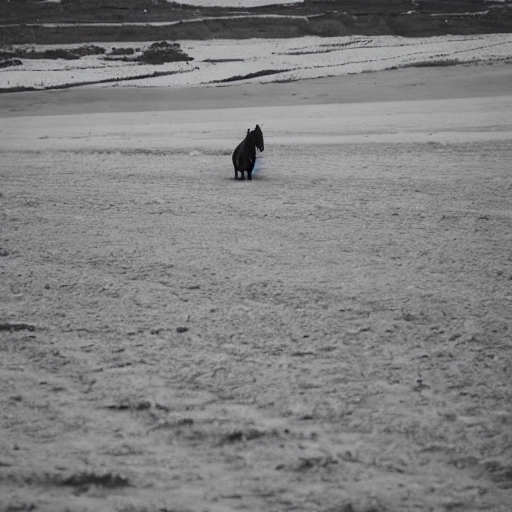
\includegraphics[width=0.28\linewidth]{img/esd_unlearn_horse.png} &
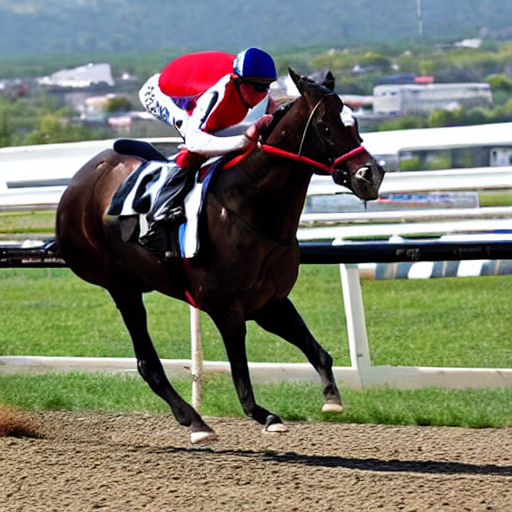
\includegraphics[width=0.28\linewidth]{img/esd_unlearn_nohorse.png} &
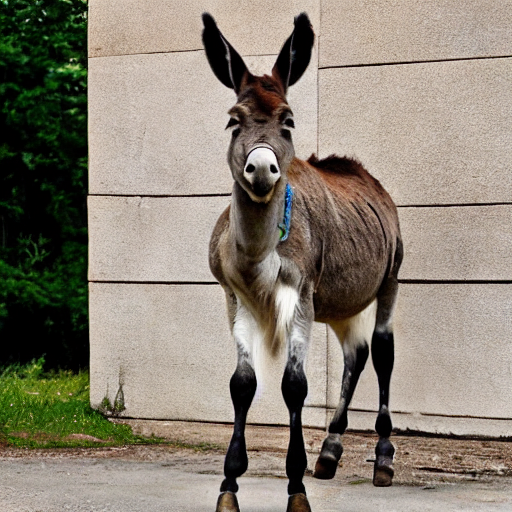
\includegraphics[width=0.28\linewidth]{img/esd_unlearn_donkey.png} \\
\textbf{STEREO} &
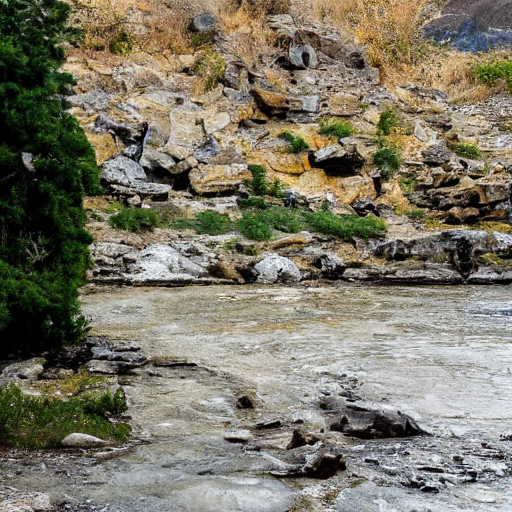
\includegraphics[width=0.28\linewidth]{img/stereo_unlearn_horse.png} &
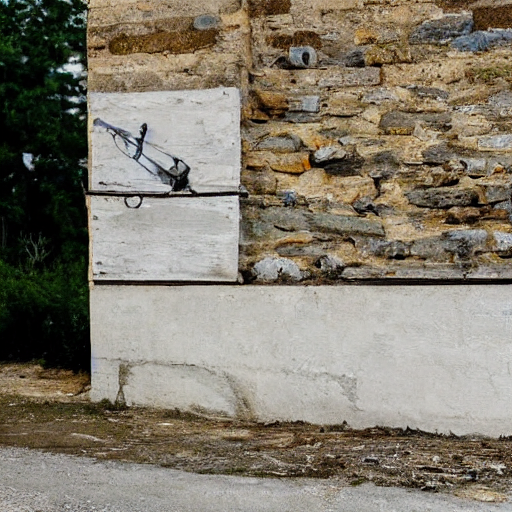
\includegraphics[width=0.28\linewidth]{img/stereo_unlearnnohorse.png} &
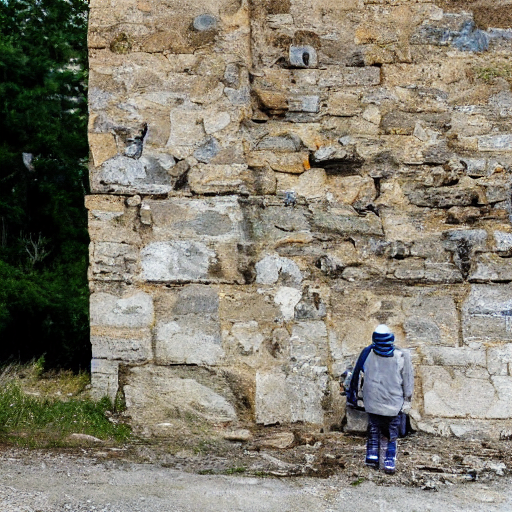
\includegraphics[width=0.28\linewidth]{img/stereo_unlearn_donkey.png} \\
\end{tabular}
\end{minipage}%
\hfill
\begin{minipage}[c]{0.38\linewidth}
\caption{
\textbf{Concept entanglement manifests as two coupled effects.}
Each row erases {horse} and is probed with three prompt types: \emph{Direct} (mentions ``\texttt{horse}''), \emph{Indirect} (uses correlated context like \texttt{jockey} but omits ``\texttt{horse}''), and \texttt{Neighbor} (semantically similar concept \texttt{donkey}). ESD leaks horses through indirect prompts but preserves donkey; STEREO suppresses leakage but destroys donkey. We formalize this duality in~\cref{sec:tradeoff}.
}
\label{fig:concept_leakage}
\end{minipage}
\end{figure*}

% \begin{figure*}[htbp]
% \centering
% \setlength{\tabcolsep}{4pt}
% \renewcommand{\arraystretch}{0.8}
% \begin{tabular}{c c c c}
%  % & \textbf{Prompt with ``horse''} & \textbf{Prompt without ``horse''} & \textbf{Prompt with ``donkey''} \\
%  & \textbf{Direct} & \textbf{Indirect} & \textbf{Neighbor} \\
% \midrule
% \textbf{ESD} &
% 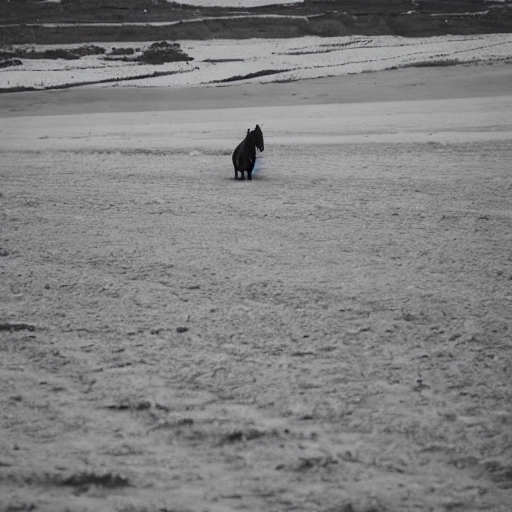
\includegraphics[width=0.15\linewidth]{img/esd_unlearn_horse.png} &
% 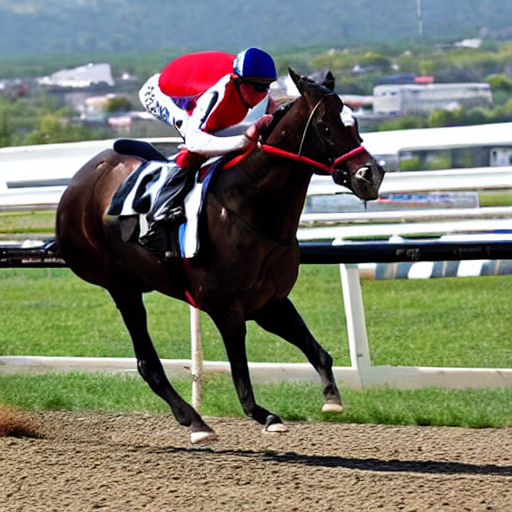
\includegraphics[width=0.15\linewidth]{img/esd_unlearn_nohorse.png} &
% 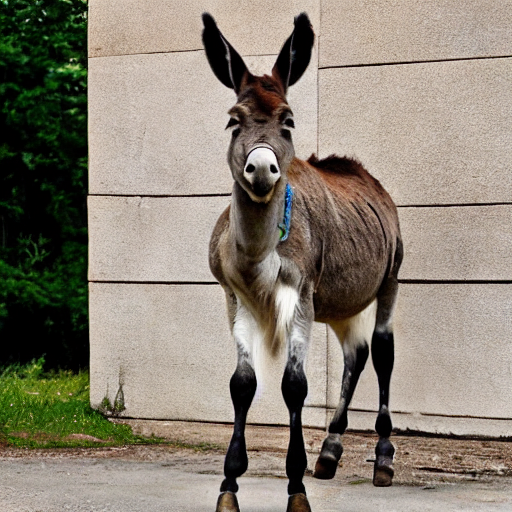
\includegraphics[width=0.15\linewidth]{img/esd_unlearn_donkey.png} \\
% % \textbf{AdvUnlearn} &
% % 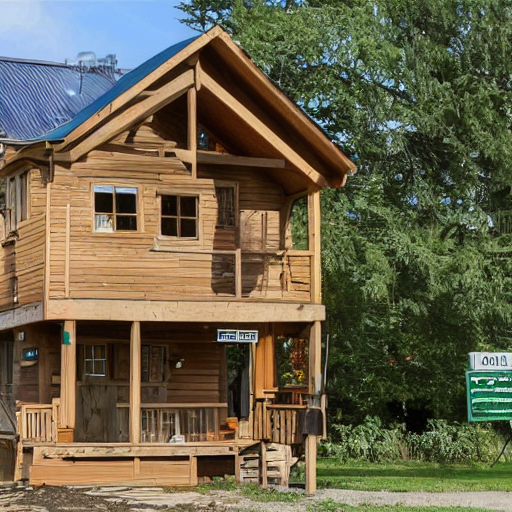
\includegraphics[width=0.13\linewidth]{img/adv_unlearn_horse.png} &
% % 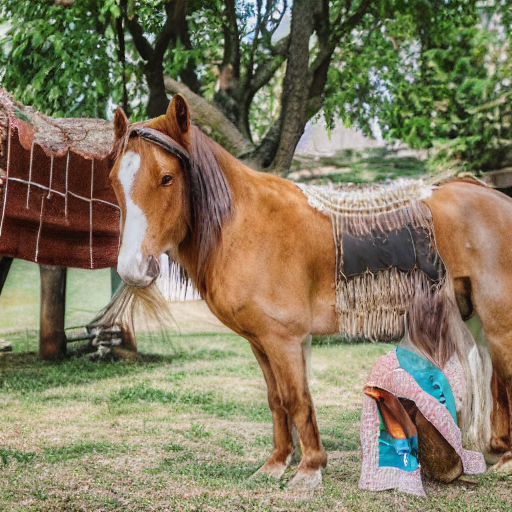
\includegraphics[width=0.13\linewidth]{img/adv_unlearn_nohorse.png} &
% % 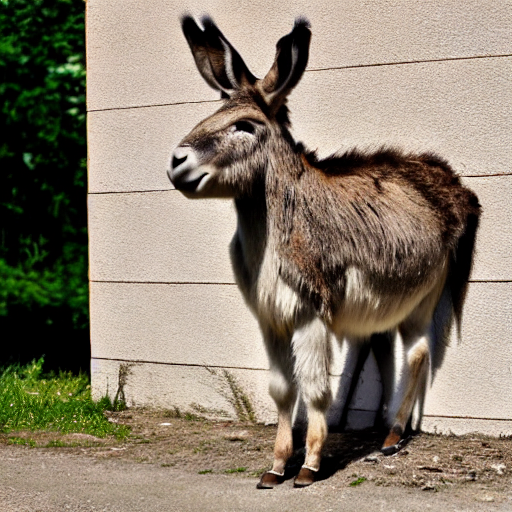
\includegraphics[width=0.13\linewidth]{img/advunlearn_unlearn_donkey.png} \\
% \textbf{STEREO} &
% 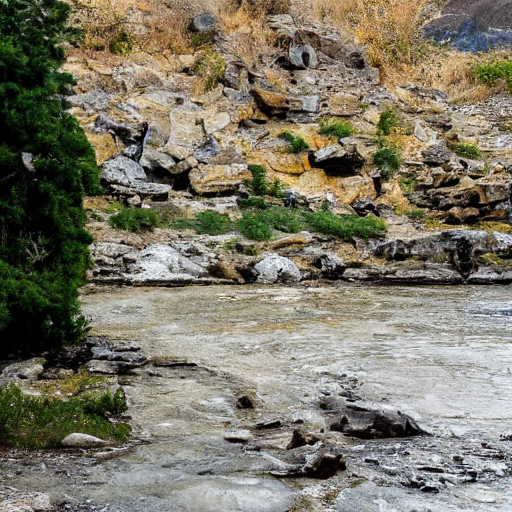
\includegraphics[width=0.15\linewidth]{img/stereo_unlearn_horse.png} &
% 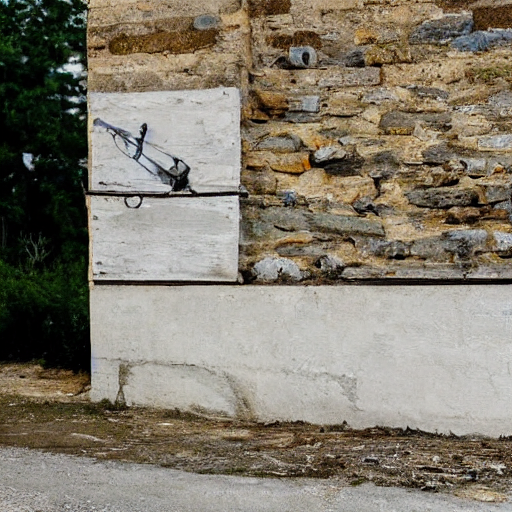
\includegraphics[width=0.15\linewidth]{img/stereo_unlearnnohorse.png} &
% 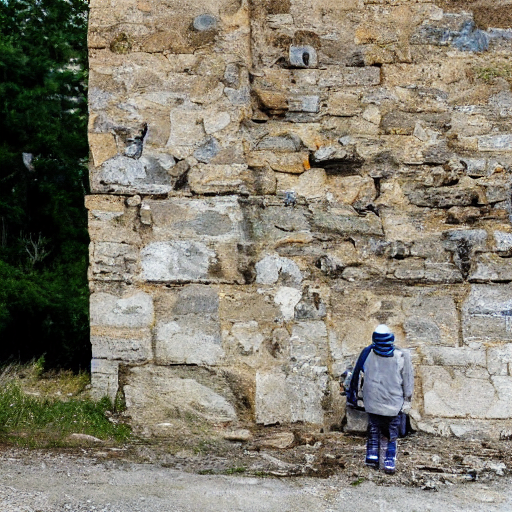
\includegraphics[width=0.15\linewidth]{img/stereo_unlearn_donkey.png} \\
% % \textbf{SAeUron} &
% % 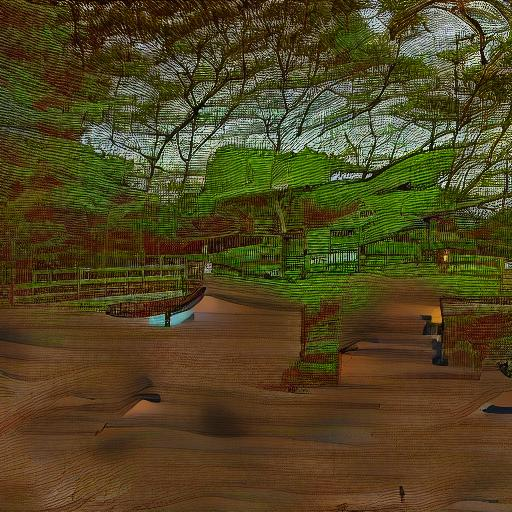
\includegraphics[width=0.13\linewidth]{img/saeuron_unlearn_horse.jpg} &
% % 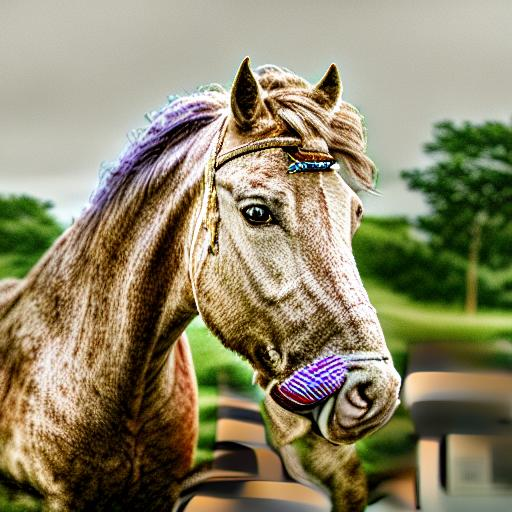
\includegraphics[width=0.13\linewidth]{img/saeuron_unlearn_nohorse.jpg} &
% % 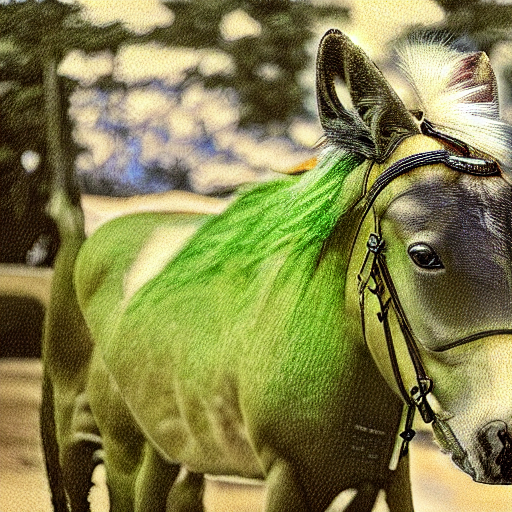
\includegraphics[width=0.13\linewidth]{img/saeuron_unlearn_donkey.png} \\
% \end{tabular}
% \caption{
% \textbf{Concept entanglement manifests as two coupled effects.}
% Each row shows the output of an unlearning method applied to erase \texttt{horse}, under three prompt types: \emph{Direct} (prompt containing ``horse''), \emph{Indirect} (prompt retaining correlated context such as \emph{jockey}, \emph{racetrack}, but omitting ``horse''), and \emph{Neighbor} (prompt for the semantically related concept \texttt{donkey})
% Localized erasure method (ESD) regenerate horses through contextual leakage in the Indirect column but preserve donkey generation in the Neighbor column. Aggressive erasure (STEREO) suppresses leakage but produces severe collateral damage on the Neighbor column, for failing to generate the donkey concept. These two effects are dual consequences of representational overlap and cannot be simultaneously avoided, as we formalize in~\cref{sec:tradeoff}. 
% % \varun{same comment as earlier figure}
% }
% \label{fig:concept_leakage}
% \end{figure*}

\begin{comment}
    \begin{figure*}[t]
\centering
\setlength{\tabcolsep}{2pt}
\begin{tabular}{c c c c c}

 & \multicolumn{2}{c}{\textbf{Prompt with ``horse''}} & \multicolumn{2}{c}{\textbf{Prompt without ``horse''}} \\

 & Original & Unlearned & Original & Unlearned \\

\midrule

\textbf{ESD} &
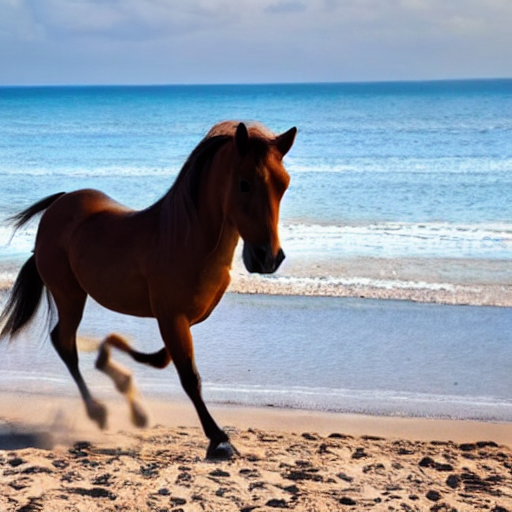
\includegraphics[width=0.13\linewidth]{img/esd_orig_horse.png} &
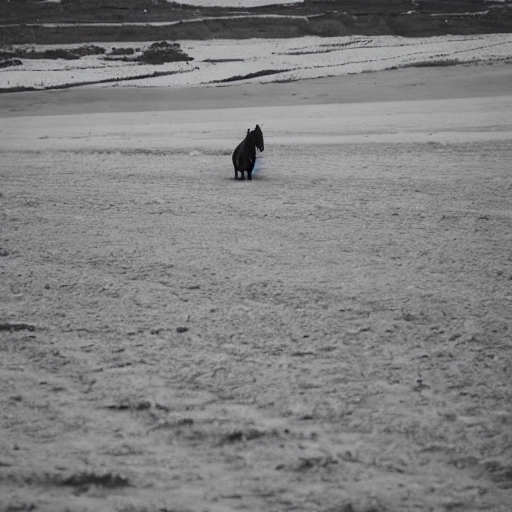
\includegraphics[width=0.13\linewidth]{img/esd_unlearn_horse.png} &
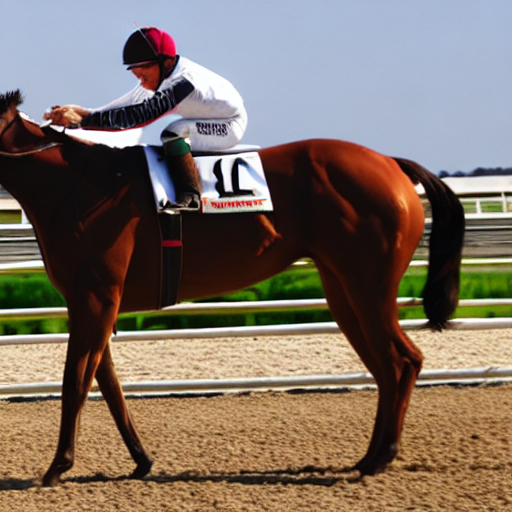
\includegraphics[width=0.13\linewidth]{img/esd_orig_nohorse.png} &
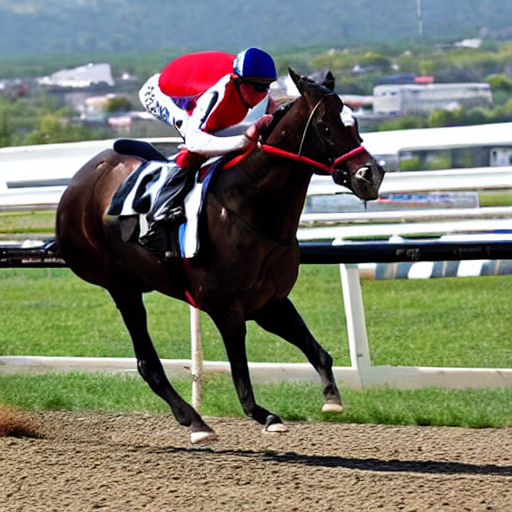
\includegraphics[width=0.13\linewidth]{img/esd_unlearn_nohorse.png} \\

\textbf{AdvUnlearn} &
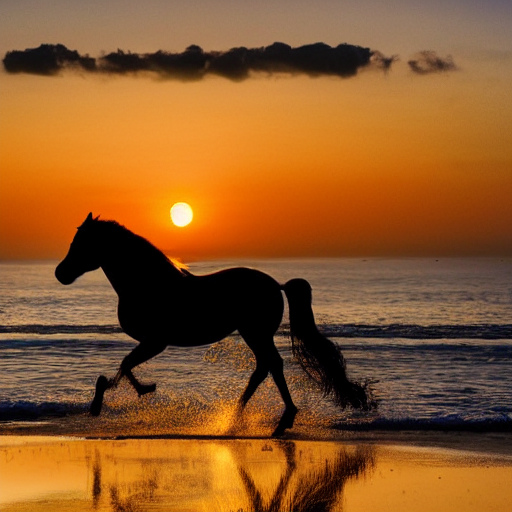
\includegraphics[width=0.13\linewidth]{img/adv_orig_horse.png} &
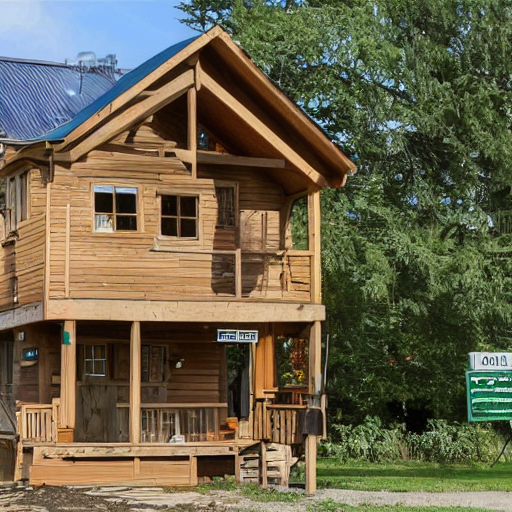
\includegraphics[width=0.13\linewidth]{img/adv_unlearn_horse.png} &
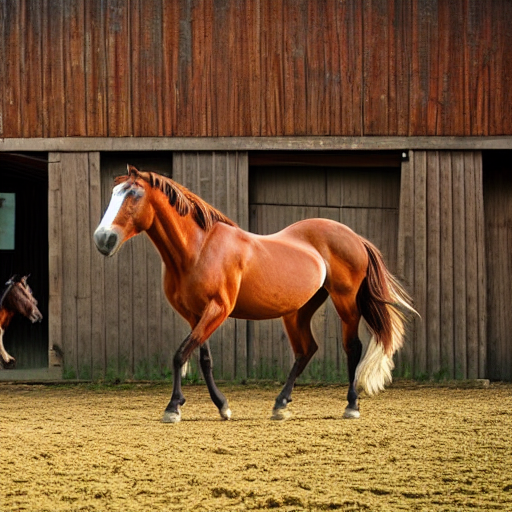
\includegraphics[width=0.13\linewidth]{img/adv_orig_nohorse.png} &
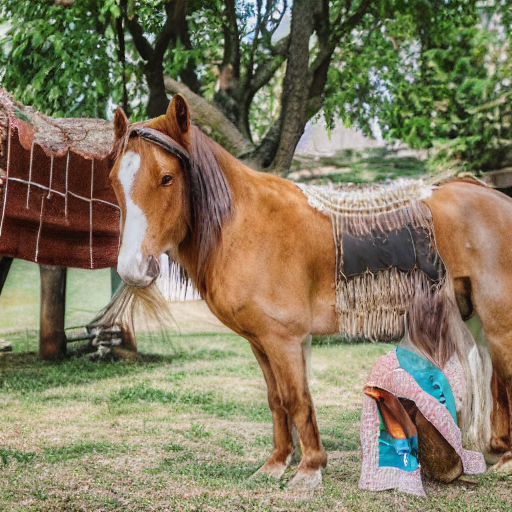
\includegraphics[width=0.13\linewidth]{img/adv_unlearn_nohorse.png} \\

\textbf{STEREO} &
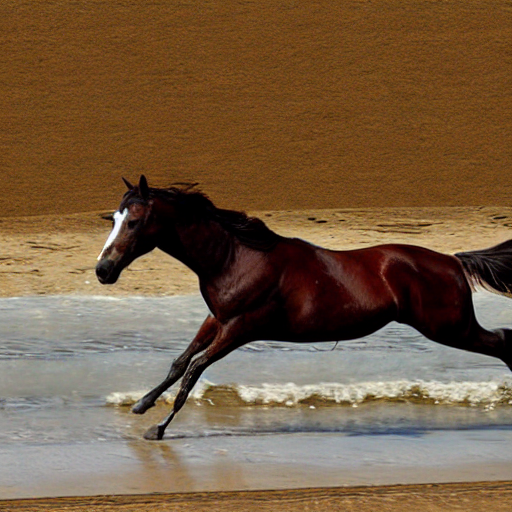
\includegraphics[width=0.13\linewidth]{img/stereo_orig_horse.png} &
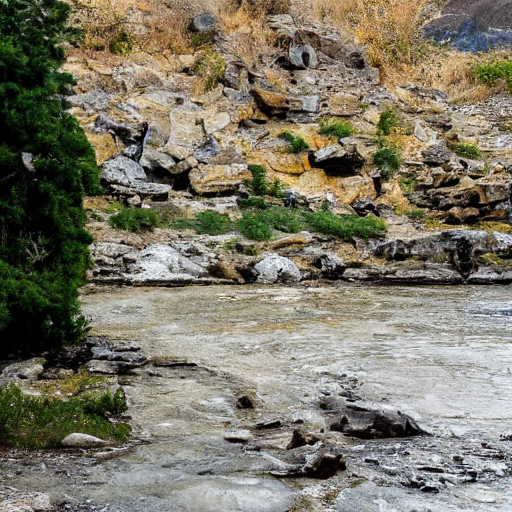
\includegraphics[width=0.13\linewidth]{img/stereo_unlearn_horse.png} &
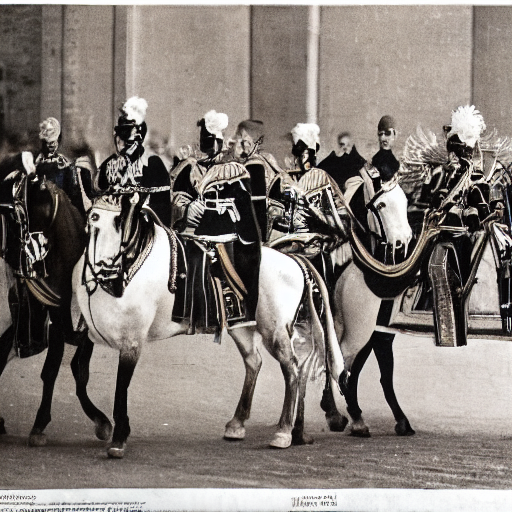
\includegraphics[width=0.13\linewidth]{img/stereo_orig_nohorse.png} &
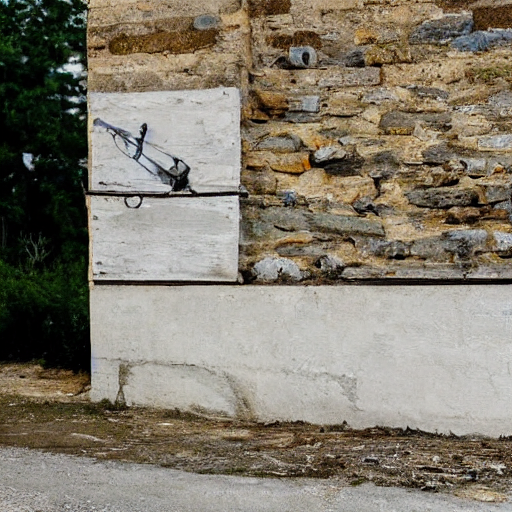
\includegraphics[width=0.13\linewidth]{img/stereo_unlearnnohorse.png} \\

\textbf{SAeUron} &
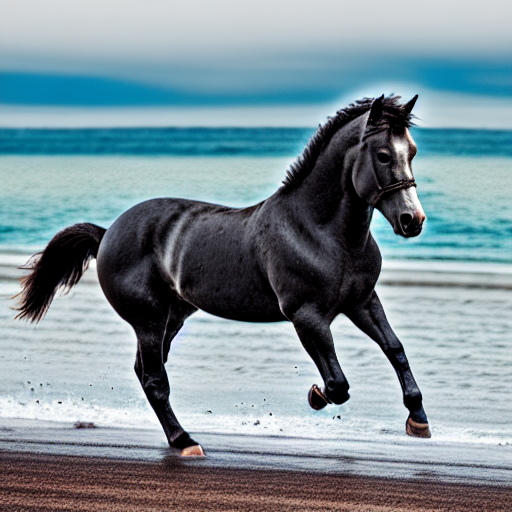
\includegraphics[width=0.13\linewidth]{img/saeuron_orig_horse.png} &
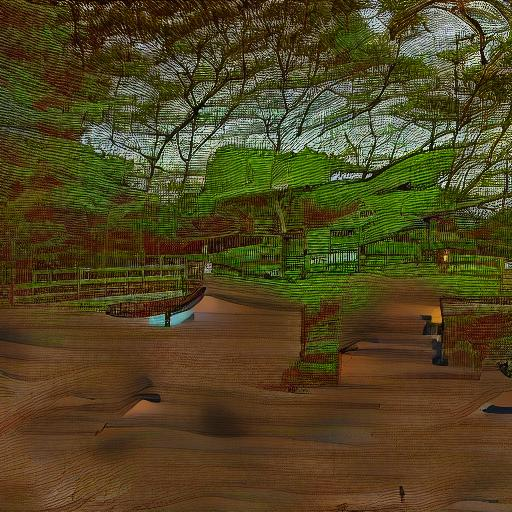
\includegraphics[width=0.13\linewidth]{img/saeuron_unlearn_horse.jpg} &
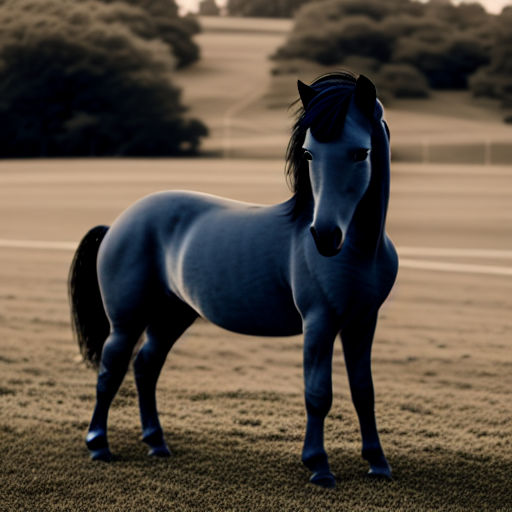
\includegraphics[width=0.13\linewidth]{img/saeuron_orig_nohorse.png} &
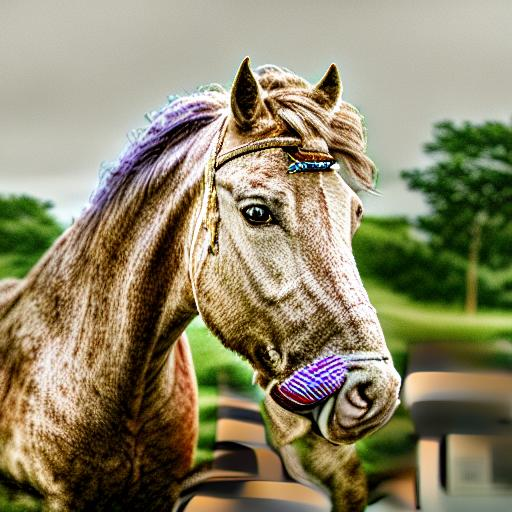
\includegraphics[width=0.13\linewidth]{img/saeuron_unlearn_nohorse.jpg} \\

\end{tabular}
\caption{
\textbf{Concept entanglement manifests as two coupled effects.}
Each row shows a different unlearning method applied to erase \texttt{horse}.
\emph{Left pair} (prompt with ``horse''): all methods successfully suppress the target concept.
\emph{Right pair} (prompt without ``horse'' but with correlated context): methods with localized erasure (ESD, SAeUron) regenerate horses through contextual leakage, while robust methods (STEREO) suppress leakage but degrades semantically neighboring concepts such as \texttt{donkey} and \texttt{zebra}. These two effects are dual consequences of representational overlap between the target concept and its semantic neighbors. %\varun{make figure much much smaller?}
}
\label{fig:concept_leakage}
\end{figure*}
\end{comment}